%*************************************************************
% Master Project                                             *
% Ing. Minerva Gabriela Vargas Gleason                       *
% IAI - Institute of Artificial Intelligence                 *
% Universität Bremen                                         *
%                                                            *
% pdfLaTex                                                   *
% Editor: TeXnicCenter                                       *
%*************************************************************


\chapter{Discussion \& Conclusion}

The aim of this work is to develop a system with a motion controller for the Boxy robot that generates trajectories that allow the robot to successfully grasp a specified object. The system must be able to decide on its own how to grasp the object. Velocity and acceleration constraints are considered by the motion controller while generating the trajectories. 

When the system receives a request of generating a trajectory to a given object, it first access the object database (section \ref{sec:db}) to retrieve the grasping poses of the object. Then, based on the distance of each grasping pose to the robot and the manipulability of both arms, selects a grasping pose and generates several trajectories. Afterwards, it repeats this process with a couple of the remaining grasping poses. Finally, the system must decide which one of the obtained trajectories is better and send it to the robot.

The system is comprised by perception, an object database, a motion controller for the Boxy robot, a trajectory evaluation service, collision detection and a projection manager that coordinates the other elements and is in charge of decision making.

From the table shown in section \ref{res:sim}, it can be seen that the initial configuration of the robot has an important influence in the success rate of the system. The motion controller tries minimize the position error of the end effector, it searches the shortest path to reach the goal. If the one or more of the arm's joints reaches joint limits in the middle of the trajectory generation, the controller won't try to move the joint in the other direction, since this would mean increasing the position and orientation error. This leads to a failed trajectory, since the controller is not able to find another solution.

However, in 26 of the 27 experiments shown in this table, table \ref{table:sim}, the controller was able to compute at least one successful trajectory. Figure \ref{fig:traj_sim} shows the result of sending a grasping command for the pancake mix bottle and the tomato sauce package. For the bottle, trajectories to three different grasping poses were planned with the right arm. For the tomato sauce, both arms reached a different grasping pose, the closest one for each.

\begin{figure}[H]
	\centering
	\begin{subfigure}[]
		{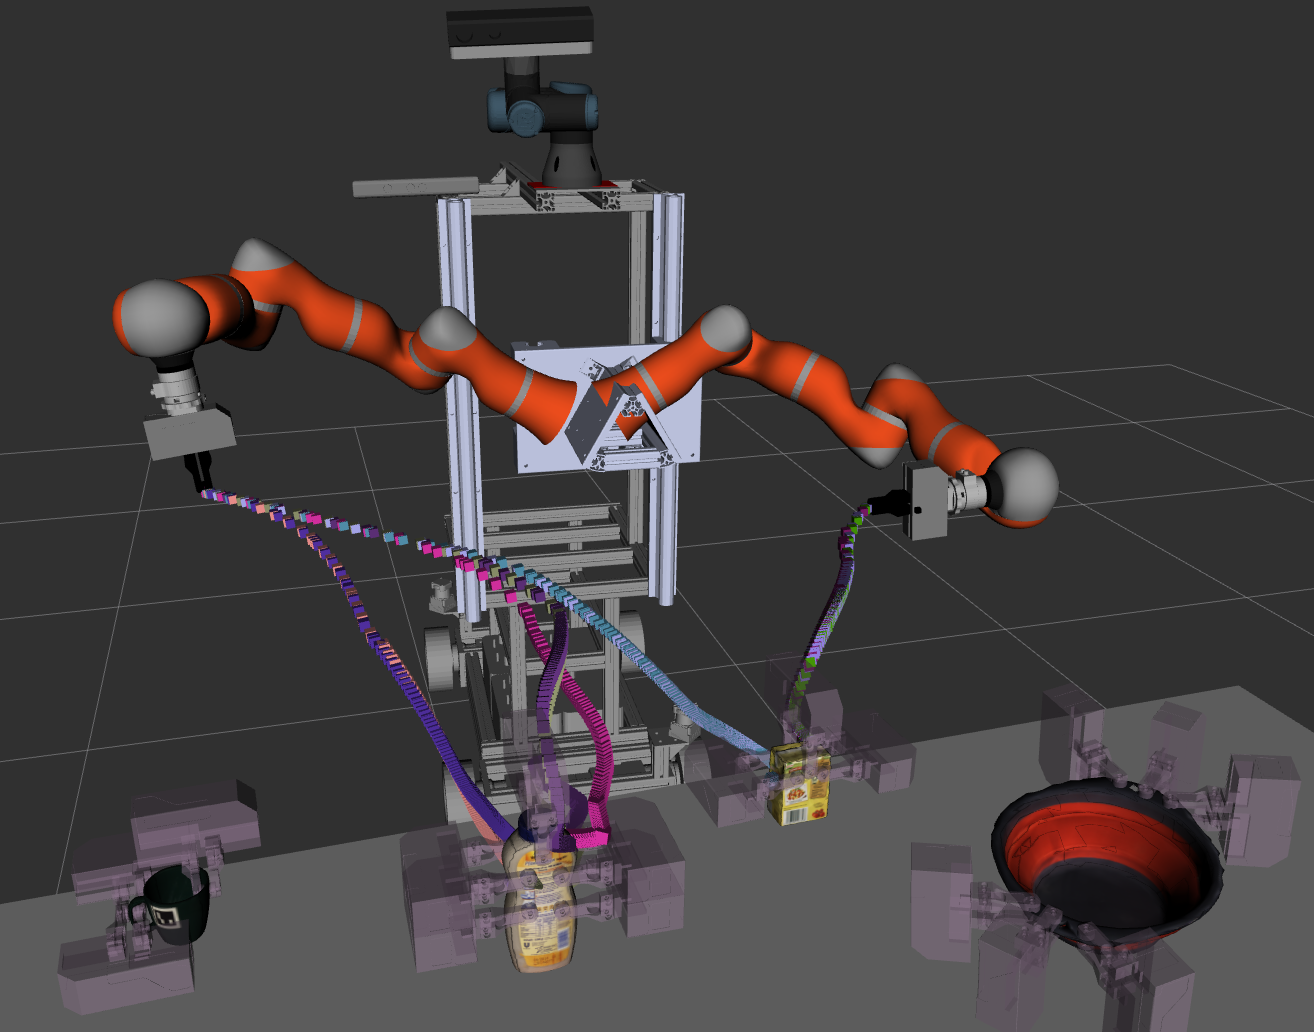
\includegraphics[width=0.46\linewidth]{sim_result.png}}
	\end{subfigure}
	\begin{subfigure}[]
		{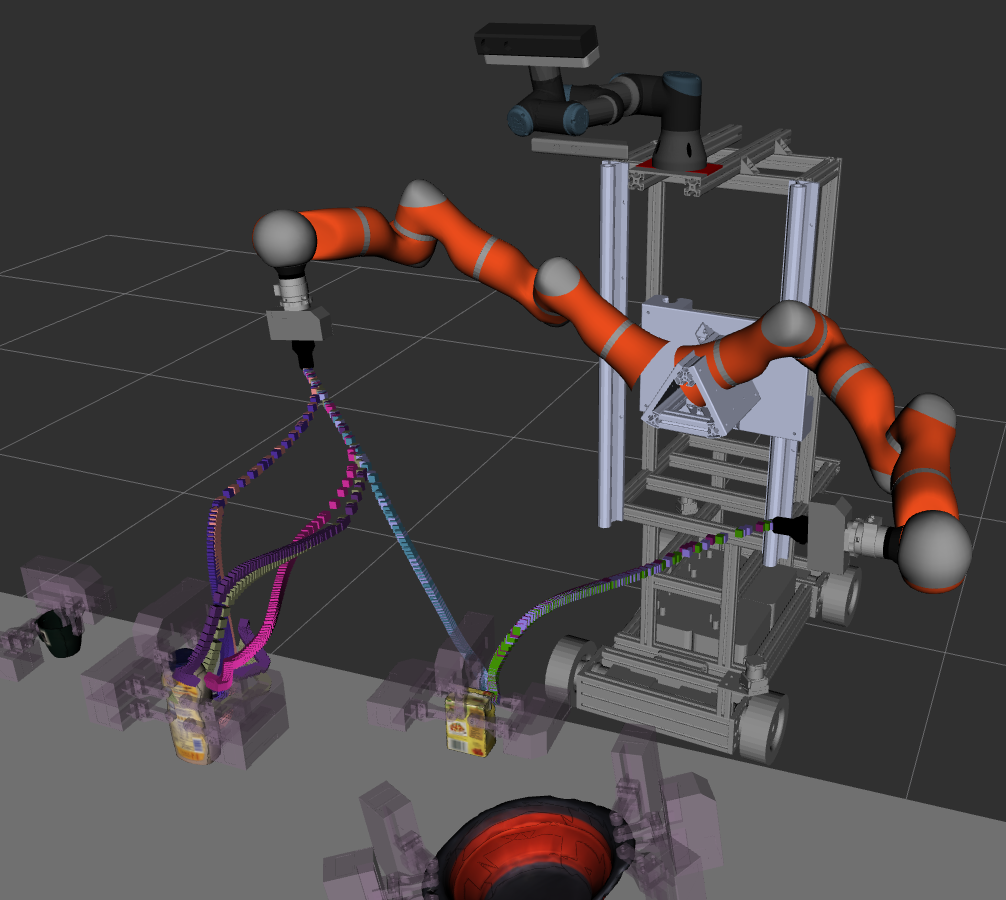
\includegraphics[width=0.4\linewidth]{sim_result2.png}}
	\end{subfigure}
	\vspace{-10pt}
	\caption[Simulated Trajectories]{Result of simulated grasping of two objects. Five trajectories per object were calculated.}
	\vspace{-15pt}
	\label{fig:traj_sim}
\end{figure}

Calculating each trajectory takes, in average, 5.9 seconds. This is the time the robot needs to execute the trajectory. On each iteration of the calculation, the controller sends a velocity command to the \textit{naive\_kinematic\_simulator}, the simulator executes this command for a small amount of time (0.01 seconds) and sends the new state back to the controller. The controller repeats this process until the robot reaches the goal position. It needs to know how long the robot must execute each command to reach the goal. This means that generating the trajectory takes as long as executing it.

However, the trajectory evaluation considerably slows down the process due to the collision detection. Checking for collisions in one trajectory lasts 14 seconds in average. This process is slow due to the amount of points in the 3D space that must be evaluated.

As a contribution in future work, lowering the time required for collision checking can be achieved by the development and implementation of improved collision models. Simplifying the geometry of all models used for collision would considerably speed up the process. Another approach could be to preload all models that might be used and then remove the ones not required before evaluating. One possible optimization is to make an interaction between generating the trajectory and evaluating it, in order to discard the trajectory as soon as a collision is found.

Some remarks I want to point out after finishing this thesis are:
\begin{itemize}
	\item Having a system with predefined grasping poses for given objects simplifies the planning of more complex grasping sequences.
	\item Fiducial markers provide a simple and reliable way of locating and identifying objects.
\end{itemize}

The results of this thesis can help researchers improve the autonomy of robots, by being able to grasp an object without having to give a specific pose as a command. This could allow a greater flexibility of the overall system and shorter the time required to plan new experiments where robots have to interact with objects.
%The research of robots that are able to perform complex task in open environments, such as collaborative work with humans, is a growing topic in the research community. These robots need the capability of analysing and understanding the information perceived by their sensors in order to define the best curse of action to fulfill a given task.
%
%Collaborative projects such as RoboHow and SAPHARI are working on improving the human-robot interaction. The main aspect addressed by these projects is obtaining a safe and intuitive interaction in collaborative tasks between humans and robots.
%
%This is done with the main goal of making human-robot interaction a reality, using a combination of cognitive reaction and a human-friendly hardware and software design, allowing collaborative work in several areas, such as assembly lines and medical surgeries, as well as every-day-tasks interaction at home.
%
%The results of this project can help researchers improve the autonomy of robots, by being able to change the orientation of their sensors as required.
%
%Some remarks I want to point out after finishing this project are:
%\begin{itemize}
%	\item Virtual links can be used to easily solve planning problems when the orientation of a sensor is involved. A virtual link can simulate the normal vector that points out of the sensor and reaches the object/area the sensor is analysing. This can be applied, for example, to orient cameras and laser sensors
%	\item MoveIt! is a powerful planning tool that allows you to select the planning algorithm that better adapts to your specific application. However, one must consider that configuring MoveIt! can take a long time if problems with the URDF are found or if the robot's drivers are not compatible with the software
%	\item When solving an already existing problem, it is important to consider which solution will be better for the user. In this case, providing two methods of setting a goal for the UR3 brings more flexibility, so the program can be used in several applications
%\end{itemize}
%
%I think there are still some areas of opportunity in MoveIt!. Currently, the software uses two files to describe the kinematic and semantic properties of the robot, these files are the URDF and the SRDF. The SRDF can be seen as an extension of the URDF, it represents the semantic information of the robot and is closely linked to the URDF. Whenever the URDF changes, the SRDF must also be updated. Unifying both files in one with the complete representation of the robot could minimize errors while programming.